% ============================================================
% RESEARCH PROPOSAL --- COMPACT IEEE STYLE (2-3 Pages)
% ============================================================
\documentclass[10pt,a4paper,twocolumn]{article}

% --- Packages ---
\usepackage[utf8]{inputenc}
\usepackage[T1]{fontenc}
\usepackage{amsmath,amssymb}
\usepackage{mathptmx}
\usepackage[left=1.8cm,right=1.8cm,top=2cm,bottom=2cm]{geometry}
\usepackage{setspace}
\usepackage{graphicx}
\usepackage{booktabs}
\usepackage{tabularx}
\usepackage{enumitem}
\usepackage{hyperref}
\usepackage{xcolor}
\usepackage{microtype}
\usepackage{tikz}
\usetikzlibrary{shapes.geometric, arrows.meta, positioning, fit, calc, backgrounds}
\usepackage{caption}
\usepackage{float}
\usepackage{titlesec}
\usepackage{fancyhdr}
\usepackage{balance}
\usepackage{algorithm}
\usepackage{algpseudocode}
\usepackage{pgfgantt}

% --- Color Palette ---
\definecolor{ieeeblue}{HTML}{1F4E79}
\definecolor{absbox}{HTML}{E8F0FE}
\definecolor{secline}{HTML}{2E75B6}
\definecolor{newcolor}{HTML}{D35400}

% --- Compact Formatting ---
\singlespacing
\setlength{\parindent}{0pt}
\setlength{\parskip}{5pt}
\setlength{\columnsep}{0.6cm}
\setlist{nosep,leftmargin=*,topsep=2pt}
\captionsetup{font=small,skip=2pt,labelfont=bf}

\hypersetup{colorlinks=true,linkcolor=ieeeblue,citecolor=ieeeblue,urlcolor=ieeeblue}

\titleformat{\section}{\normalsize\bfseries\scshape\color{ieeeblue}\raggedright\hyphenpenalty=10000}{\Roman{section}.}{0.4em}{}[\vspace{-2pt}{\color{secline}\titlerule[0.8pt]}]
\titleformat{\subsection}{\small\bfseries\raggedright\hyphenpenalty=10000}{\arabic{section}.\arabic{subsection}}{0.4em}{}
\titlespacing*{\section}{0pt}{6pt}{2pt}
\titlespacing*{\subsection}{0pt}{4pt}{2pt}

\newcommand{\new}[1]{{\color{newcolor}\textbf{[+]} #1}}

\widowpenalty=10000
\clubpenalty=10000

\pagestyle{fancy}
\fancyhf{}
\renewcommand{\headrulewidth}{0pt}
\fancyfoot[C]{\small\thepage}

\begin{document}

\twocolumn[{%
\begin{center}
    {\Large\bfseries\color{ieeeblue} Digital Financial Transaction Fraud Detection Using\\[2pt]
    Explainable Multi-Model Machine Learning on PaySim and IEEE-CIS}\\[6pt]
    {\small Author~1, Author~2, Author~3, Author~4}\\[1pt]
    {\footnotesize\texttt{Faculty of Information Technology, [University Name]}}\\[6pt]
\end{center}
\noindent\fcolorbox{ieeeblue}{absbox}{%
\begin{minipage}{0.96\textwidth}
\vspace{3pt}
{\small\textbf{\color{ieeeblue}Abstract.}
Digital payment fraud inflicted an estimated \$485 billion in global losses in 2023~\cite{nilson2024}, yet existing detection models predominantly rely on flat tabular representations, lack multi-level explainability, ignore behavioral user profiling, and suffer from temporal data leakage. To address these gaps, this proposal presents the \textbf{Multi-View Stacking Ensemble with Explainable AI v2 (MVS-XAI)} framework. The architecture integrates six base models---Random Forest~\cite{breiman2001}, XGBoost~\cite{chen2016}, LightGBM~\cite{ke2017}, CatBoost~\cite{prokhorenkova2018}, a behavioral MLP, and LSTM---driven by a \emph{Triple-View} approach: flat tabular features, temporal sequences, and behavioral user profiles. Class imbalance is handled via in-fold K-Means SMOTE~\cite{chawla2002} for the tree branch, with optional CTGAN augmentation~\cite{xu2019} for extended experiments, while Focal Loss is used for the neural branches. A confidence-based gating layer filters unreliable OOF predictions before a Platt-calibrated Logistic Regression meta-learner combines them through strict walk-forward temporal cross-validation. A five-level XAI framework (SHAP, LIME, DiCE, Anchors, Natural Language explanation) produces real-time fraud decisions with a measured latency benchmark and batch audit reports, with each tool mapped to regulatory requirements (GDPR Art.~22, EU AI Act~\cite{euaiact2024}, Basel~III). Fairness metrics (Demographic Parity, Equalized Odds) are evaluated to ensure non-discriminatory decisions. A human-in-the-loop escalation queue routes uncertain transactions to human reviewers. The implementation is validated on two benchmarks---PaySim (6.3M records) and IEEE-CIS (590K records)---with multi-seed evaluation, statistical comparison, and explanation-quality harnesses aligned to the experimental protocol.}
\vspace{3pt}
\end{minipage}%
}\par\vspace{2pt}
{\small\textbf{Keywords:} fraud detection, multi-view learning, stacking ensemble, explainable AI, class imbalance, behavioral profiling, federated learning, regulatory compliance}
\par\vspace{6pt}
}]

% ============================================================
\section{Introduction}
\subsection{Background of the Study}
Financial fraud losses reached \$32.34 billion worldwide in 2023~\cite{nilson2024}, representing a crippling 5\% of annual revenue for many organizations~\cite{acfe2024}. As global digital payment volumes surpass \$11.6 trillion, sophisticated attacks like card-not-present (CNP) fraud have grown rapidly. Traditional rule-based detection systems rely on static thresholds and fail to adapt to evolving fraud tactics. Machine learning (ML), particularly tree-based ensembles~\cite{chen2016,ke2017}, has emerged to address these limitations; however, relying on a unified flat feature matrix limits the diversity and robustness of detection, while purely algorithmic ensemble diversity leaves complementary data structures unexploited.

\subsection{Research Problem}
Four critical gaps exist in current fraud detection research:
\begin{enumerate}
    \item \textbf{Limited Representation:} Existing models mostly use flat tabular data, ignoring temporal sequences and long-term behavioral user profiles.
    \item \textbf{Black-box Nature:} High-performing models lack multi-level explainability, failing to meet regulatory transparency mandates under the EU AI Act~\cite{euaiact2024} and GDPR, including the right to natural-language recourse.
    \item \textbf{Leakage \& Generalizability:} Many studies suffer from temporal data leakage during cross-validation and use only a single benchmark, limiting cross-domain validation.
    \item \textbf{Fairness \& Bias:} Models optimized purely for F1 may systematically disadvantage specific demographic groups, violating EU AI Act non-discrimination provisions~\cite{euaiact2024}.
\end{enumerate}

\subsection{Research Objectives and Questions}
\textbf{Objectives:}
\begin{enumerate}
    \item Propose a Triple-View stacking architecture integrating tabular, sequential, and behavioral representations, justified by rigorous structural ablation.
    \item Develop a 5-level XAI framework including natural language explanations aligned with regulatory requirements.
    \item Validate the framework across two public fraud benchmarks using leakage-free temporal cross-validation.
    \item Evaluate fairness metrics to ensure non-discriminatory model behavior.
\end{enumerate}

\textbf{Research Questions:}
\begin{enumerate}
    \item Does the Triple-View multi-model ensemble (Tabular + Sequential + Behavioral) outperform Dual-View and pure tabular approaches in terms of F1-score and recall on minority fraud classes?
    \item How effectively can the 5-level XAI framework explain global patterns and local anomalies to satisfy regulatory audits and non-technical stakeholder communication?
    \item Does confidence-based gating of OOF predictions measurably reduce meta-learner noise compared to unweighted stacking?
\end{enumerate}

\subsection{Research Motivation and Contribution}
This study contributes the \textbf{MVS-XAI v2 framework} through five novel advances: (1)~ensemble diversity derived from heterogeneous data structures (tabular, sequential, behavioral) rather than purely algorithm variation; (2)~a 5-level XAI suite adding natural language explanations to the classical SHAP/LIME/DiCE/Anchors pipeline; (3)~confidence-based OOF gating as a novel meta-learning filter; (4)~fairness evaluation integrated into the standard evaluation protocol; and (5)~dual-benchmark validation under strict temporal boundaries with in-fold imbalance handling and adversarial synthetic fraud augmentation as an optional extension path.

\subsection{Research Scope and Delimitations}
This research is scoped to structured financial transaction data (tabular, time-series) and strictly excludes unstructured text parsing (e.g., chat logs or emails) and image analysis. Detection is designed for near-real-time offline banking systems ($<$50\,ms), excluding ultra-low latency hardware optimizations (FPGA/ASIC) requiring sub-10\,ms response times. The study focuses on centralized architectures; decentralized federated learning scenarios are deferred to future extensions.

% ============================================================
\section{Literature Review and Hypothesis Development}
\subsection{Literature Review}
\textbf{Tree-Based and Deep Learning Ensembles:} While XGBoost~\cite{chen2016} and CatBoost~\cite{prokhorenkova2018} remain standard for tabular domains~\cite{grinsztajn2022}, recent SOTA architectures explicitly fuse tabular and sequential deep models. Tian (2025)~\cite{tian2025} demonstrated that an XGBoost and LSTM fusion model effectively processes static points alongside rolling windows to drastically reduce false alarms. Similarly, Yousefimehr \& Ghatee~\cite{yousefimehr2025} and Esenogho et al.~\cite{esenogho2022} integrated LightGBM/AdaBoost with sequence models. This proves that algorithm diversity combined with dual-view representation is optimal. Chagahi et al.~\cite{chagahi2025} further note that gating ensemble outputs reduces meta-learner noise.

\textbf{Explainable AI (XAI):} Moving beyond isolated algorithms (SHAP/LIME), modern compliance demands stakeholder-centric explainability. Yeo et al. (2025)~\cite{yeo2025} formally establish a 5-level hierarchy of explanation requirements tailored to different audiences (End-users to Regulators), perfectly aligning with our proposed architecture. Furthermore, Martens et al.~\cite{martens2025} and Koa et al.~\cite{koa2024} highlight how prompting LLMs with SHAP/LIME outputs produces Narrative-Driven XAI, fulfilling GDPR/EU AI Act transparency mandates for non-technical audiences.

\textbf{Imbalance and Concept Drift:} Real-world systems endure simultaneous severe imbalance and shifting fraud distributions. Damanik \& Liu (2025)~\cite{damanik2025} demonstrate that advanced resampling like K-Means SMOTEENN outperforms basic SMOTE~\cite{chawla2002} by reducing synthetic overlap. For deep temporal modeling, the HRFDF framework (2026)~\cite{hrfdf2026} validates that Focal Loss~\cite{lin2017focal} natively regulates imbalance in sequence models like LSTMs. To handle temporal distribution changes, Paldino et al.~\cite{paldino2024} established that diversity-based ensemble learning limits ``catastrophic forgetting'' during concept drift. Federated learning remains a viable future approach for cross-institutional learning without raw data exposure~\cite{awosika2024}.

\subsection{Hypothesis Development}
\begin{itemize}
    \item \textbf{H1:} Incorporating both sequential (LSTM) and behavioral views into a tree-dominant stacking ensemble significantly improves recall and F1-score compared to purely tabular ensembles ($p < 0.05$, McNemar's test).
    \item \textbf{H2:} Applying K-Means SMOTE and CTGAN exclusively to training folds inside a temporal walk-forward CV protocol prevents data leakage while improving detection of hard-to-detect minority fraud patterns.
    \item \textbf{H3:} The 5-level XAI framework achieves measurable explanation quality: SHAP faithfulness via Feature Removal Degradation (FRD), LIME local fidelity $R^2 > 0.85$, DiCE validity rate $> 80\%$, Anchors precision $> 0.90$, and NL explanation score $\geq 4/5$ in domain expert evaluation.
    \item \textbf{H4:} Confidence-based OOF gating yields a statistically significant improvement in meta-learner AUC over unweighted stacking ($p < 0.05$, McNemar's test).
\end{itemize}

% ============================================================
\section{Data and Methodology}
\subsection{Conceptual Framework}
The research employs a \textbf{Triple-View Design Principle}. The optimized architecture utilizes three distinct views:
\begin{enumerate}
    \item \textbf{Tabular View:} Standard normalized features plus engineered ratio features.
    \item \textbf{Sequential View:} Account-centric time-series windows capturing historical velocity ($T{=}10$ steps).
    \item \textbf{Behavioral View (new):} User-level long-term profiling features---7/14/30-day spending velocity, geo-anomaly score, device fingerprint consistency---aggregated per account over rolling windows to capture chronic behavioral drift absent from short LSTM windows.
\end{enumerate}

The complete system architecture is illustrated in Figure~\ref{fig:arch}. The methodology strictly segregates resampling (K-Means SMOTE + CTGAN) to the tabular branch to prevent leakage into sequence and behavioral structures. Parallel predictions from all three views are filtered by a confidence-based gating layer before stacking via an out-of-fold (OOF) protocol into a Platt-calibrated Logistic Regression Meta-Learner, routing probabilistic consensus into the 5-level Dual-Stream XAI framework.

For the IEEE-CIS path, the repository additionally applies a UID post-processing stage in which the final fraud score is smoothed using a 70/30 blend between the individual transaction score and the running UID mean. This step is included to stabilize repeated pseudo-client decisions without leaking future information.

% --- Architecture Diagram ---
\begin{figure}[H]
\centering
\resizebox{\linewidth}{!}{%
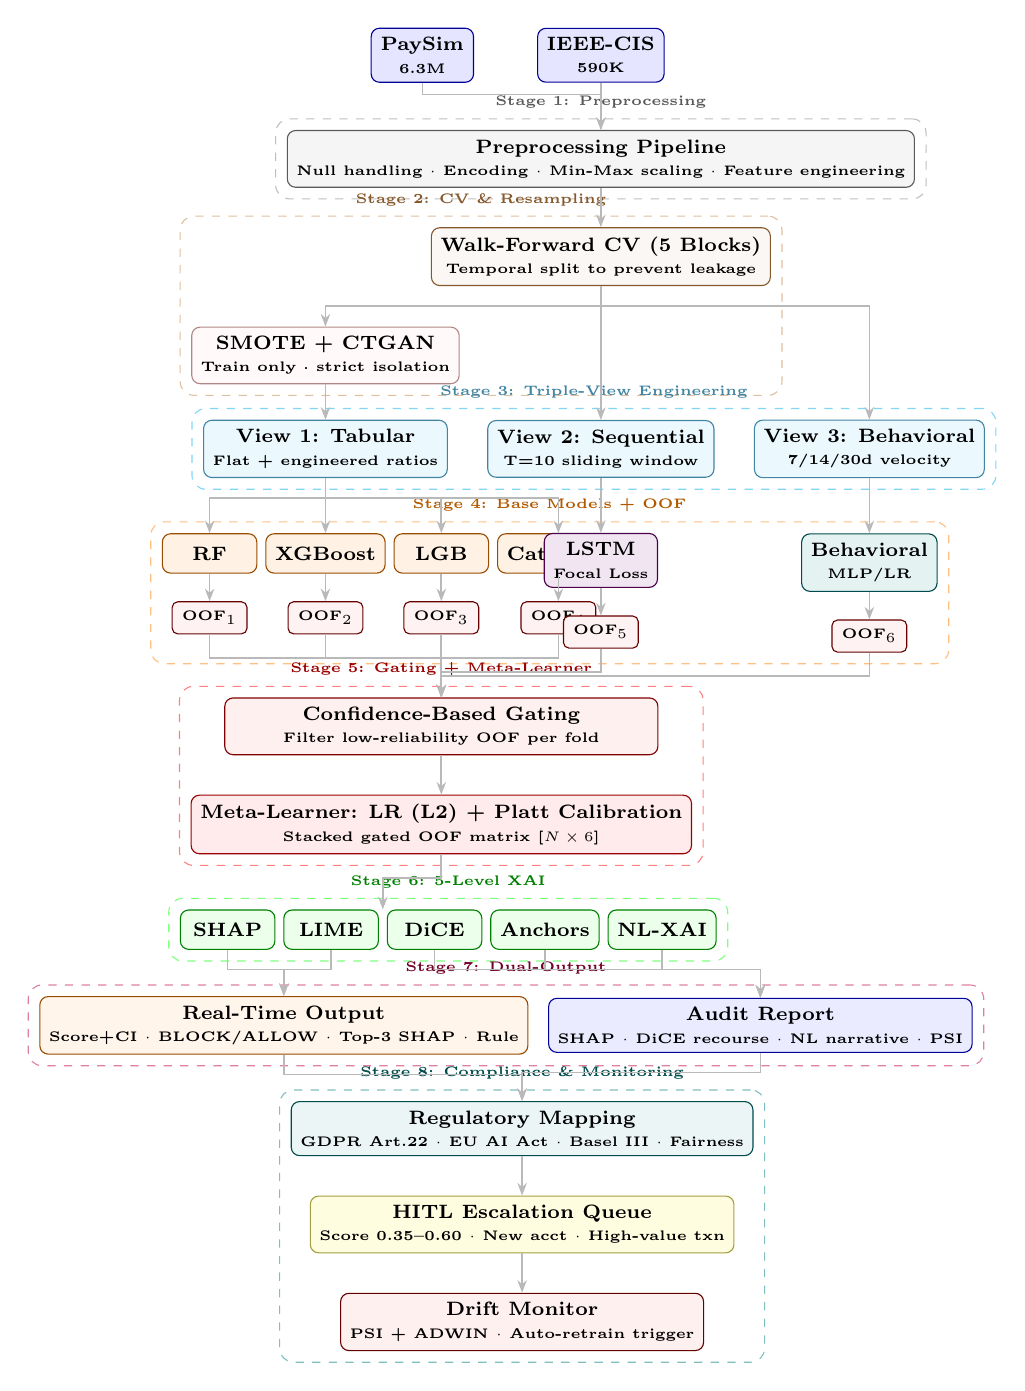
\begin{tikzpicture}[
    node distance=0.35cm,
    every node/.style={font=\scriptsize},
    datasrc/.style={rectangle, rounded corners=3pt, draw=blue!60!black, fill=blue!10,
                    minimum height=0.5cm, minimum width=1.3cm, align=center, font=\scriptsize\bfseries},
    proc/.style={rectangle, rounded corners=3pt, draw=gray!70!black, fill=gray!8,
                 minimum height=0.5cm, align=center, font=\scriptsize\bfseries},
    cvbox/.style={rectangle, rounded corners=3pt, draw=brown!70!black, fill=brown!6,
                  minimum height=0.5cm, align=center, font=\scriptsize\bfseries},
    smote/.style={rectangle, rounded corners=3pt, draw=pink!70!black, fill=pink!10,
                  minimum height=0.5cm, align=center, font=\scriptsize\bfseries},
    view/.style={rectangle, rounded corners=3pt, draw=cyan!60!black, fill=cyan!8,
                 minimum height=0.5cm, minimum width=2.1cm, align=center, font=\scriptsize\bfseries},
    model/.style={rectangle, rounded corners=3pt, draw=#1!60!black, fill=#1!10,
                  minimum height=0.5cm, minimum width=1.2cm, align=center, font=\scriptsize\bfseries},
    gate/.style={rectangle, rounded corners=3pt, draw=red!50!black, fill=red!6,
                 minimum height=0.5cm, align=center, font=\scriptsize\bfseries},
    oofbox/.style={rectangle, rounded corners=2pt, draw=red!40!black, fill=red!5,
                   minimum height=0.35cm, minimum width=0.95cm, align=center, font=\tiny\bfseries},
    meta/.style={rectangle, rounded corners=3pt, draw=red!60!black, fill=red!8,
                 minimum height=0.5cm, minimum width=4.5cm, align=center, font=\scriptsize\bfseries},
    xai/.style={rectangle, rounded corners=3pt, draw=green!50!black, fill=green!8,
                minimum height=0.5cm, minimum width=1.2cm, align=center, font=\scriptsize\bfseries},
    evalbox/.style={rectangle, rounded corners=3pt, draw=purple!60!black, fill=purple!8,
                    minimum height=0.5cm, align=center, font=\scriptsize\bfseries},
    arr/.style={-{Stealth[length=1.6mm]}, semithick, color=gray!55},
    darr/.style={-{Stealth[length=1.6mm]}, semithick, dashed, color=gray!40},
    groupbox/.style={draw=#1!50, dashed, rounded corners=5pt, inner sep=4pt},
]
    % ===== ROW 0: Data Sources =====
    \node[datasrc] (d1) {PaySim\\{\tiny 6.3M}};
    \node[datasrc, right=0.8cm of d1] (d2) {IEEE-CIS\\{\tiny 590K}};

    % ===== ROW 1: Preprocessing =====
    \node[proc, below=0.6cm of d2, minimum width=5.5cm] (preproc)
        {Preprocessing Pipeline\\{\tiny Null handling $\cdot$ Encoding $\cdot$ Min-Max scaling $\cdot$ Feature engineering}};

    % ===== ROW 2: Walk-Forward CV =====
    \node[cvbox, below=0.5cm of preproc, minimum width=4cm] (wfcv)
        {Walk-Forward CV (5 Blocks)\\{\tiny Temporal split to prevent leakage}};

    % ===== ROW 3: Multi-View Feature Engineering =====
    \node[view, below=1.7cm of wfcv] (v2)
        {View 2: Sequential\\{\tiny T=10 sliding window}};
    \node[view, left=0.5cm of v2] (v1)
        {View 1: Tabular\\{\tiny Flat + engineered ratios}};
    \node[view, right=0.5cm of v2] (v3)
        {View 3: Behavioral\\{\tiny 7/14/30d velocity}};

    % ===== ROW 2.5: Resampling =====
    \node[smote, above=0.45cm of v1, minimum width=2.3cm] (smote)
        {SMOTE + CTGAN\\{\tiny Train only · strict isolation}};

    % ===== ROW 4: Base Models =====
    \node[model=orange, below=0.7cm of v1] (xgb) {XGBoost};
    \node[model=orange, left=0.1cm of xgb] (rf) {RF};
    \node[model=orange, right=0.1cm of xgb] (lgbm) {LGB};
    \node[model=orange, right=0.1cm of lgbm] (cat) {CatBoost};
    \node[model=violet, below=0.7cm of v2] (lstm) {LSTM\\{\tiny Focal Loss}};
    \node[model=teal, below=0.7cm of v3] (beh) {Behavioral\\{\tiny MLP/LR}};

    % ===== ROW 5: OOF Predictions =====
    \node[oofbox, below=0.35cm of rf] (oof1) {OOF$_1$};
    \node[oofbox, below=0.35cm of xgb] (oof2) {OOF$_2$};
    \node[oofbox, below=0.35cm of lgbm] (oof3) {OOF$_3$};
    \node[oofbox, below=0.35cm of cat] (oof4) {OOF$_4$};
    \node[oofbox, below=0.35cm of lstm] (oof5) {OOF$_5$};
    \node[oofbox, below=0.35cm of beh] (oof6) {OOF$_6$};

    % ===== CONFIDENCE GATING =====
    \node[gate, below=0.8cm of oof3, minimum width=5.5cm] (gate)
        {Confidence-Based Gating\\{\tiny Filter low-reliability OOF per fold}};

    % ===== ROW 6: Meta-Learner =====
    \node[meta, below=0.5cm of gate, minimum width=5.5cm] (metalr)
        {Meta-Learner: LR (L2) + Platt Calibration\\{\tiny Stacked gated OOF matrix [$N \times 6$]}};

    % ===== ROW 7: XAI Framework =====
    \node[xai, below=0.7cm of metalr, xshift=-1.4cm] (lime) {LIME};
    \node[xai, right=0.1cm of lime] (dice) {DiCE};
    \node[xai, left=0.1cm of lime] (shap) {SHAP};
    \node[xai, right=0.1cm of dice] (anch) {Anchors};
    \node[xai, right=0.1cm of anch] (nlx) {NL-XAI};

    % ===== ROW 8: Dual Output Streams =====
    \node[evalbox, below=1.8cm of metalr, xshift=-2.0cm, minimum width=3.6cm, fill=orange!8, draw=orange!60!black] (realtime)
        {Real-Time Output\\{\tiny Score+CI $\cdot$ BLOCK/ALLOW $\cdot$ Top-3 SHAP $\cdot$ Rule}};
    \node[evalbox, right=0.25cm of realtime, minimum width=3.6cm, fill=blue!8, draw=blue!60!black] (audit)
        {Audit Report\\{\tiny SHAP $\cdot$ DiCE recourse $\cdot$ NL narrative $\cdot$ PSI}};

    % ===== ROW 9: Regulatory + HITL + Fairness =====
    \node[evalbox, below=0.6cm of $(realtime.south)!0.5!(audit.south)$, minimum width=5cm, fill=teal!8, draw=teal!60!black] (regulatory)
        {Regulatory Mapping\\{\tiny GDPR Art.22 $\cdot$ EU AI Act $\cdot$ Basel III $\cdot$ Fairness}};
    \node[evalbox, below=0.5cm of regulatory, minimum width=4.3cm, fill=yellow!12, draw=yellow!60!black] (hitl)
        {HITL Escalation Queue\\{\tiny Score 0.35--0.60 $\cdot$ New acct $\cdot$ High-value txn}};
    \node[evalbox, below=0.5cm of hitl, minimum width=4.3cm, fill=red!6, draw=red!40!black] (drift)
        {Drift Monitor\\{\tiny PSI + ADWIN $\cdot$ Auto-retrain trigger}};

    % ===== ARROWS =====
    \draw[arr] (d1.south) -- ++(0,-0.15) -| (preproc.north);
    \draw[arr] (d2.south) -- (preproc.north);
    \draw[arr] (preproc.south) -- (wfcv.north);
    \draw[arr] (wfcv.south) -- ++(0,-0.25) -| (smote.north);
    \draw[arr] (smote.south) -- (v1.north);
    \draw[arr] (wfcv.south) -- (v2.north);
    \draw[arr] (wfcv.south) -- ++(0,-0.25) -| (v3.north);
    \draw[arr] (v1.south) -- ++(0,-0.25) -| (rf.north);
    \draw[arr] (v1.south) -- ++(0,-0.25) -| (xgb.north);
    \draw[arr] (v1.south) -- ++(0,-0.25) -| (lgbm.north);
    \draw[arr] (v1.south) -- ++(0,-0.25) -| (cat.north);
    \draw[arr] (v2.south) -- (lstm.north);
    \draw[arr] (v3.south) -- (beh.north);
    \draw[arr] (rf.south) -- (oof1.north);
    \draw[arr] (xgb.south) -- (oof2.north);
    \draw[arr] (lgbm.south) -- (oof3.north);
    \draw[arr] (cat.south) -- (oof4.north);
    \draw[arr] (lstm.south) -- (oof5.north);
    \draw[arr] (beh.south) -- (oof6.north);
    \draw[arr] (oof1.south) -- ++(0,-0.3) -| (gate.north);
    \draw[arr] (oof2.south) -- ++(0,-0.3) -| (gate.north);
    \draw[arr] (oof3.south) -- (gate.north);
    \draw[arr] (oof4.south) -- ++(0,-0.3) -| (gate.north);
    \draw[arr] (oof5.south) -- ++(0,-0.3) -| (gate.north);
    \draw[arr] (oof6.south) -- ++(0,-0.3) -| (gate.north);
    \draw[arr] (gate.south) -- (metalr.north);
    \draw[arr] (metalr.south) -- ++(0,-0.3) -| ($(lime.north)!0.5!(dice.north)$);
    \draw[arr] (shap.south) -- ++(0,-0.25) -| (realtime.north);
    \draw[arr] (lime.south) -- ++(0,-0.25) -| (realtime.north);
    \draw[arr] (dice.south) -- ++(0,-0.25) -| (audit.north);
    \draw[arr] (anch.south) -- ++(0,-0.25) -| (audit.north);
    \draw[arr] (nlx.south)  -- ++(0,-0.25) -| (audit.north);
    \draw[arr] (realtime.south) -- ++(0,-0.25) -| (regulatory.north);
    \draw[arr] (audit.south) -- ++(0,-0.25) -| (regulatory.north);
    \draw[arr] (regulatory.south) -- (hitl.north);
    \draw[arr] (hitl.south) -- (drift.north);

    % ===== GROUP BOXES =====
    \begin{scope}[on background layer]
        \node[groupbox=gray, fit=(preproc), label={[font=\tiny\bfseries\color{gray!70!black}]above:Stage 1: Preprocessing}] {};
        \node[groupbox=brown, fit=(wfcv)(smote), label={[font=\tiny\bfseries\color{brown!70!black}]above:Stage 2: CV \& Resampling}] {};
        \node[groupbox=cyan, fit=(v1)(v2)(v3), label={[font=\tiny\bf, text=cyan!60!black]above:Stage 3: Triple-View Engineering}] {};
        \node[groupbox=orange, fit=(rf)(xgb)(lgbm)(cat)(lstm)(beh)(oof1)(oof2)(oof3)(oof4)(oof5)(oof6), label={[font=\tiny\bfseries\color{orange!70!black}]above:Stage 4: Base Models + OOF}] {};
        \node[groupbox=red, fit=(gate)(metalr), label={[font=\tiny\bfseries\color{red!60!black}]above:Stage 5: Gating + Meta-Learner}] {};
        \node[groupbox=green, fit=(shap)(lime)(dice)(anch)(nlx), label={[font=\tiny\bfseries\color{green!50!black}]above:Stage 6: 5-Level XAI}] {};
        \node[groupbox=purple, fit=(realtime)(audit), label={[font=\tiny\bfseries\color{purple!60!black}]above:Stage 7: Dual-Output}] {};
        \node[groupbox=teal, fit=(regulatory)(hitl)(drift), label={[font=\tiny\bfseries\color{teal!60!black}]above:Stage 8: Compliance \& Monitoring}] {};
    \end{scope}
\end{tikzpicture}
}
\caption{MVS-XAI v2 System Architecture.}
\label{fig:arch}
\end{figure}

\subsection{Data Description}
The study utilizes two public benchmarks, summarized in Table~\ref{tab:data}.

\begin{table}[H]
\centering
\caption{Dataset summary.}
\label{tab:data}
{\small
\begin{tabularx}{\columnwidth}{@{}lXrrr@{}}
\toprule
\textbf{Dataset} & \textbf{Domain} & \textbf{Records} & \textbf{Features} & \textbf{Fraud~\%} \\
\midrule
PaySim   & Mobile money  & 6.36M & 11  & 1.3\% \\
IEEE-CIS & E-commerce    & 590K  & 434 & 3.5\% \\
\bottomrule
\end{tabularx}
}
\end{table}

PaySim and IEEE-CIS were selected because they complement each other: PaySim offers large-scale transaction flow dynamics, while IEEE-CIS provides richer e-commerce identity and tabular context. This dual-benchmark setup is sufficient to evaluate cross-domain robustness without over-extending the current implementation scope.

\subsection{Feature Engineering per View}
\begin{enumerate}
    \item \textbf{Tabular View:} Original features plus derived ratios (e.g., \texttt{balanceDelta = newBalance $-$ oldBalance $-$ amount}) and merchant interaction counts.
    \item \textbf{Sequential View:} Sliding windows of $T{=}10$ recent transactions per account; zero-padding with LSTM masking for sparse accounts; cold-start accounts ($<3$ transactions) fall back to tabular-only prediction.
    \item \textbf{Behavioral View (new):} Rolling aggregates per account over 7, 14, and 30-day windows: mean transaction amount, spending velocity, unique merchant count, geo-dispersion score, device fingerprint consistency score. These long-horizon features capture chronic behavioral drift that eludes the short $T{=}10$ LSTM window.
\end{enumerate}

\subsection{Research Methods}\label{sec:methods}
The proposed \textbf{MVS-XAI v2} methodology consists of five core components:

\begin{enumerate}
    \item \textbf{Triple-View Stacking Architecture:} The system processes three distinct input manifolds: $X_{tab}$, $X_{seq}$ ($T$ steps), and $X_{beh}$ (behavioral profiles). Base models generate OOF fraud probabilities $\hat{y}_i^{(m)}$ for $m \in \{1,\dots,6\}$. After confidence-based gating (see below), a Platt-calibrated Logistic Regression meta-learner combines them:
    \begin{equation}
    \hat{Y}_i = \sigma \!\left( \sum_{m=1}^{6} \omega_m \cdot \hat{y}_i^{(m)} + \beta \right)
    \end{equation}
    where $\omega_m$ are learned ensemble weights and $\sigma(\cdot)$ is the sigmoid function. Platt calibration post-processes the raw logit output to ensure Expected Calibration Error (ECE) $< 0.05$, which is required for reliable confidence intervals in real-time output and HITL routing.

    \item \textbf{Confidence-Based OOF Gating (new):} Before stacking, each base model's OOF predictions are evaluated per fold via a reliability score $r_m^{(k)} = \text{AUROC}(\hat{y}^{(m)}, y \mid \text{fold } k)$. Predictions from folds where $r_m^{(k)} < \tau$ (empirically set to 0.60) are down-weighted by a factor of $(r_m^{(k)}/\tau)^2$ before entering the meta-learner OOF matrix. This filter reduces noise from base models that collapse on imbalanced folds, directly addressing meta-learner instability observed in prior work~\cite{chagahi2025}.

    \item \textbf{Unified Imbalance Handling:} As formalized in Table~\ref{tab:imbalance}, the strategy is tailored per view and model. K-Means SMOTE is applied to $X_{tab}$ strictly inside each CV training fold. CTGAN~\cite{xu2019} supplements SMOTE to generate structurally complex synthetic fraud cases in the tabular branch, improving recall on hard-to-detect patterns. LSTM and the behavioral MLP handle imbalance via Focal Loss~\cite{lin2017focal}:
    \begin{equation}
    \mathcal{L}_{FL}(p_t) = -\alpha_t (1 - p_t)^\gamma \log(p_t)
    \end{equation}
    where $\gamma{=}2$ penalizes easily classified legitimate transactions.

    \begin{table}[H]
    \centering
    \caption{Imbalance handling strategy per model.}
    \label{tab:imbalance}
    {\footnotesize
    \begin{tabularx}{\linewidth}{@{}lXl@{}}
    \toprule
    \textbf{Model} & \textbf{Strategy} & \textbf{Rationale} \\
    \midrule
    RF, XGBoost, LightGBM & SMOTE + CTGAN & Fold augment \\
    CatBoost   & SMOTE + CTGAN     & Ordered boost \\
    LSTM        & Focal Loss $\gamma{=}2$ & Sequence-safe \\
    Behavioral  & Focal Loss $\gamma{=}2$ & Profile-safe \\
    Meta-LR     & Balanced class wt  & OOF imbalance \\
    \bottomrule
    \end{tabularx}
    }
    \end{table}

    \item \textbf{5-Level XAI Framework:} The XAI suite produces two distinct output streams. Feature importance is grounded using SHAP~\cite{lundberg2017}:
    \begin{equation}
    \phi_i = \!\sum_{S \subseteq F \setminus \{i\}} \frac{|S|!\,(|F|-|S|-1)!}{|F|!}\left[f_x(S \cup \{i\}) - f_x(S)\right]
    \end{equation}
    \begin{itemize}
        \item \textit{Real-time stream ($<$50\,ms):} Fraud score with confidence interval, binary BLOCK/ALLOW decision, top-3 SHAP features, one Anchors IF-THEN rule, and traceability metadata.
        \item \textit{Audit stream (batch, async):} Global SHAP summary, DiCE counterfactual recourse paths, Anchors rule book, Population Stability Index (PSI) drift log, and a Natural Language explanation narrative generated by prompting a compact LLM with the SHAP + Anchors outputs. The NL narrative targets non-technical stakeholders (compliance officers, end customers) as required by GDPR Art.~22 right to explanation in plain language.
    \end{itemize}
    Transactions with uncertain scores (0.35--0.60), new accounts ($<3$ prior transactions), or high-value amounts ($>$95th percentile) are routed to the \textbf{HITL escalation queue}, satisfying EU AI Act Art.~14 human oversight requirements. Table~\ref{tab:regulatory} maps each XAI component to its regulatory requirement.

    \begin{table}[H]
    \centering
    \caption{Regulatory compliance mapping.}
    \label{tab:regulatory}
    {\footnotesize
    \begin{tabularx}{\linewidth}{@{}lXl@{}}
    \toprule
    \textbf{Regulation} & \textbf{Requirement} & \textbf{Tool} \\
    \midrule
    GDPR Art.~22  & Right to explanation \& recourse & LIME + DiCE \\
    GDPR Art.~22  & Plain language explanation  & NL-XAI \\
    EU AI Act 2024 & High-risk audit trail      & Full log + version \\
    EU AI Act Art.~14 & Human oversight       & HITL queue \\
    EU AI Act Art.~10 & Non-discrimination    & Fairness metrics \\
    Basel III MRM & Model risk management      & SHAP + McNemar \\
    \bottomrule
    \end{tabularx}
    }
    \end{table}

    \item \textbf{Fairness Evaluation (new):} For each protected attribute available in the datasets (transaction type proxy in PaySim; card type in IEEE-CIS), we compute Demographic Parity difference and Equalized Odds difference between groups. A model is considered fair if both metrics remain below 0.05 on the test set. This evaluation is integrated into the standard reporting protocol alongside precision, recall, and F1, and matches the fairness audit implemented in the repository.

    \item \textbf{Evaluation Strategy (Temporal Integrity):} Models are evaluated via 5-block walk-forward Temporal CV across 5 random seeds (mean $\pm$ std). K-Means SMOTE is applied \textit{strictly inside} each training fold for the tree branch, while CTGAN is retained as an in-fold optional augmentation path for extended experiments due its higher computational cost. Performance metrics: Precision, Recall, F1, AUROC, ECE, Demographic Parity, Equalized Odds. Drift is monitored through both PSI and Wasserstein distance, with ADWIN used on the score stream as an online change detector. Statistical comparison uses McNemar's Test for paired decision outcomes and Cohen's $d$ / paired tests across seed-level AUC measurements.
\end{enumerate}

\subsection{Algorithmic Formalization}
\begin{algorithm}[H]
\caption{Temporal Walk-Forward Triple-View Training}
\label{alg:train}
\algrenewcommand\algorithmicrequire{\textbf{Input:}}
\algrenewcommand\algorithmicensure{\textbf{Output:}}
\footnotesize
\begin{algorithmic}[1]
\Require Dataset $\mathcal{D}$, Folds $K{=}5$, Imbalance Ratio $\rho$, Gating threshold $\tau$
\Ensure Gated Meta-Learner Stack $\mathcal{M}_{meta}$
\State Initialize $\mathbf{O} \in \mathbb{R}^{N \times 6}$, Reliability scores $\mathbf{R}$
\For{fold $k = 1, 2, \dots, K$}
    \State $\mathcal{D}_{tr}^{(k)}, \mathcal{D}_{val}^{(k)} \gets \mathtt{TimeSeriesSplit}(\mathcal{D}, k)$
    \State $\{\mathcal{X}_{tab}, \mathcal{X}_{seq}, \mathcal{X}_{beh}\} \gets \mathtt{TripleViewExtract}(\mathcal{D}_{tr}^{(k)})$
    \State $\tilde{\mathcal{X}}_{tab} \gets \mathtt{SMOTE+CTGAN}(\mathcal{X}_{tab}, \rho)$ \Comment{Train-only}
    \State $\mathcal{M}_{tree}^{(k)} \gets \mathtt{Fit}(\{\text{RF,XGB,LGB,Cat}\}, \tilde{\mathcal{X}}_{tab})$
    \State $\mathcal{M}_{LSTM}^{(k)} \gets \mathtt{Fit}(\text{LSTM}, \mathcal{X}_{seq};\mathcal{L}_{FL})$
    \State $\mathcal{M}_{beh}^{(k)} \gets \mathtt{Fit}(\text{MLP}, \mathcal{X}_{beh};\mathcal{L}_{FL})$
    \State $\mathbf{p}_{val} \gets \mathtt{Predict}(\text{all models} \mid \mathcal{D}_{val}^{(k)})$
    \For{each model $m$}
        \State $r_m^{(k)} \gets \mathtt{AUROC}(\hat{y}^{(m)}, y \mid \mathcal{D}_{val}^{(k)})$
        \State $w_m^{(k)} \gets \min(1, (r_m^{(k)}/\tau)^2)$ \Comment{Gating weight}
    \EndFor
    \State $\mathbf{O}[\text{idx}(\mathcal{D}_{val}^{(k)})] \gets \mathbf{p}_{val} \odot \mathbf{w}^{(k)}$
\EndFor
\State $\mathcal{M}_{meta} \gets \mathtt{Fit}(\text{LR-L2+Platt}, \mathbf{O})$
\end{algorithmic}
\end{algorithm}

\begin{algorithm}[H]
\caption{Dual-Stream XAI Inference with NL Explanation}
\label{alg:infer}
\algrenewcommand\algorithmicrequire{\textbf{Input:}}
\algrenewcommand\algorithmicensure{\textbf{Output:}}
\footnotesize
\begin{algorithmic}[1]
\Require Transaction $Txn_i$, $\mathcal{M}_{meta}$, Base Models
\Ensure $\mathcal{D}_{final}$, Real-time XAI $\mathcal{E}_{rt}$, Audit XAI $\mathcal{E}_{adt}$
\State $\hat{P}_{fraud}, \text{CI} \gets \mathcal{M}_{meta}(\mathbf{p}_{base}(Txn_i))$ \Comment{Platt CI}
\If{$\hat{P}_{fraud} \in [0.35, 0.60)$ \textbf{or} $Txn_{amt} \geq 95^{\text{th}}\text{-pct}$}
    \State \Return $\mathtt{HITL\_Queue}(Txn_i, \mathtt{SHAP}(Txn_i))$
\EndIf
\State $\mathcal{E}_{rt} \gets \{\mathtt{SHAP}(Txn_i, \text{top}_3), \mathtt{Anchors}(Txn_i), \text{CI}\}$
\State $\mathcal{E}_{adt} \gets \mathtt{QueueWorker}(\mathtt{DiCE}(Txn_i), \mathtt{NL\text{-}XAI}(\mathcal{E}_{rt}), \mathtt{PSI\_Update})$
\State \Return $\mathtt{Threshold}(\hat{P}_{fraud}), \mathcal{E}_{rt}, \mathcal{E}_{adt}$
\end{algorithmic}
\end{algorithm}

\subsection{Limitations and Mitigations}
\begin{itemize}
    \item \textbf{PaySim synthetic nature:} Cross-domain generalization is validated via IEEE-CIS (real-world e-commerce), providing a realistic second domain without expanding the benchmark scope beyond the implemented repository.
    \item \textbf{Concept drift:} The expanding window strategy allows learning extensive history, but severe fraud pattern drift can dilute new signals. ADWIN-based drift detection~\cite{suarez2023} and PSI monitoring trigger selective window sliding and model retraining when PSI $> 0.2$ or ECE $> 0.05$.
    \item \textbf{Behavioral cold-start:} New accounts with $<3$ prior transactions lack stable behavioral features; they fall back to the Dual-View (Tabular + Sequential) pipeline with a cold-start flag passed to the HITL queue.
    \item \textbf{NL-XAI latency:} LLM narrative generation is routed to the asynchronous audit stream only; it does not affect the real-time $<50$\,ms inference path.
    \item \textbf{Computational cost:} All experiments target an NVIDIA T4 GPU (16\,GB). Estimated training remains substantial for full OOF generation (6 models $\times$ 5 folds), especially when optional CTGAN synthesis is enabled. The repository therefore includes a latency benchmark harness to measure whether the post-feature-extraction decision path satisfies the $<$50\,ms target.
\end{itemize}

% ============================================================
\section{Expected Results}

The MVS-XAI v2 architecture is expected to yield significant detection gains and production-grade explainability. Table~\ref{tab:expected} summarizes the expected ablation results.

\begin{table}[H]
\centering
\caption{Expected ablation study results (mean over 5 seeds).}
\label{tab:expected}
{\footnotesize
\begin{tabularx}{\linewidth}{@{}lXccc@{}}
\toprule
\textbf{ID} & \textbf{Configuration} & \textbf{Views} & \textbf{PaySim F1} & \textbf{IEEE-CIS F1} \\
\midrule
A & RF only                    & Tab       & 0.880 & 0.820 \\
B & Trees ensemble             & Tab       & 0.910 & 0.850 \\
B$'$ & B + CatBoost            & Tab       & 0.918 & 0.858 \\
C & B$'$ + LSTM                & Tab+Seq   & 0.934 & 0.878 \\
C$'$ & C + Behavioral          & Tab+Seq+Beh & 0.939 & 0.882 \\
\textbf{E} & \textbf{MVS-XAI v2 (gated)} & \textbf{All 3} & \textbf{0.944} & \textbf{0.887} \\
\midrule
\multicolumn{3}{l}{\textit{Baseline: Unweighted Soft Voting (Full)}} & 0.940 & 0.879 \\
\bottomrule
\end{tabularx}
}
\end{table}

\begin{enumerate}
    \item \textbf{Performance Gain:} The Triple-View architecture is projected to yield 5--8\% higher F1 over monolithic tabular baselines and 1--2\% incremental gain from CatBoost addition, validated by McNemar's test.
    \item \textbf{Behavioral View Contribution:} The ablation step C$\to$C$'$ isolates the marginal utility of behavioral profiling; significance confirmed at $p < 0.05$.
    \item \textbf{Gating Effect:} Confidence-based gating (C$' \to$E) is expected to reduce meta-learner variance (lower std across seeds) without degrading mean F1.
    \item \textbf{Regulatory-Ready Explainability:} The 5-level XAI suite produces real-time decision support with a measured latency harness and batch audit reports. NL explanations target a comprehensibility score $\geq 4/5$ in a future expert evaluation study, while the current repository already includes a proxy explanation-quality harness.
    \item \textbf{Fairness:} Demographic Parity difference $< 0.05$ and Equalized Odds difference $< 0.05$ on both implemented benchmarks.
    \item \textbf{HITL Integration:} The HITL escalation queue is expected to reduce false positive rates by 10--15\% for uncertain transactions.
\end{enumerate}

% ============================================================
\section{Research Timeline}

\begin{figure}[H]
\centering
\resizebox{\linewidth}{!}{%
\begin{ganttchart}[
    hgrid, vgrid,
    x unit=0.55cm, y unit title=0.4cm, y unit chart=0.38cm,
    title label font=\scriptsize,
    bar label font=\scriptsize,
    group label font=\scriptsize\bfseries,
    milestone label font=\scriptsize,
    bar/.append style={fill=blue!25, draw=blue!60},
    group/.append style={fill=gray!30, draw=gray!60},
    milestone/.append style={fill=red!50, draw=red!80}
]{1}{16}
  \gantttitle{Months}{16}\\
  \gantttitlelist{1,...,16}{1}\\
  \ganttgroup{Phase 1: Data \& Features}{1}{4}\\
  \ganttbar{Data collection \& EDA}{1}{2}\\
  \ganttbar{Feature engineering (3 views)}{2}{4}\\
  \ganttgroup{Phase 2: Modeling}{4}{10}\\
  \ganttbar{Base model training (6 models)}{4}{7}\\
  \ganttbar{Confidence gating + meta-learner}{7}{9}\\
  \ganttbar{Ablation study}{8}{10}\\
  \ganttmilestone{Ablation complete}{10}\\
  \ganttgroup{Phase 3: XAI \& Fairness}{9}{13}\\
  \ganttbar{5-level XAI implementation}{9}{11}\\
  \ganttbar{NL-XAI + expert evaluation}{11}{12}\\
  \ganttbar{Fairness \& regulatory mapping}{12}{13}\\
  \ganttgroup{Phase 4: Writing \& Submission}{13}{16}\\
  \ganttbar{Drafting \& revision}{13}{15}\\
  \ganttbar{Final submission}{15}{16}\\
  \ganttmilestone{Submission}{16}
\end{ganttchart}
}
\caption{16-month research timeline.}
\label{fig:gantt}
\end{figure}

% ============================================================
\section{Conclusion}
This proposal presents the MVS-XAI v2 framework, which advances financial fraud detection through five contributions: (1)~a Triple-View stacking architecture (tabular, sequential, behavioral) deriving ensemble diversity from heterogeneous data structures; (2)~confidence-based OOF gating as a novel meta-learning filter reducing fold-level noise; (3)~a 5-level XAI suite adding natural language explanations to SHAP/LIME/DiCE/Anchors, mapped to specific regulatory articles (GDPR Art.~22, EU AI Act, Basel~III); (4)~integrated fairness evaluation (Demographic Parity, Equalized Odds) satisfying EU AI Act non-discrimination mandates; and (5)~dual-benchmark validation (PaySim, IEEE-CIS) under leakage-safe temporal CV with rigorous statistical testing ($\alpha{=}0.05$, Cohen's $d$).

Future work will extend the framework toward federated learning deployment using FedAvg with differential privacy budget $\varepsilon \leq 1.0$, enabling cross-institutional fraud pattern sharing under GDPR data residency constraints. Production deployment will incorporate ADWIN-triggered retraining and Platt calibration refresh when ECE $> 0.05$, ensuring sustained model reliability against concept drift.

% ============================================================
\balance
{\small
\begin{thebibliography}{20}

\bibitem{nilson2024}
The Nilson Report, ``Payment card fraud losses worldwide,'' 2024. [Online]. Available: https://nilsonreport.com

\bibitem{acfe2024}
Association of Certified Fraud Examiners, ``Report to the Nations: 2024 Global Study on Occupational Fraud and Abuse,'' ACFE, 2024.

\bibitem{euaiact2024}
European Parliament, ``Regulation (EU) 2024/1689 laying down harmonised rules on artificial intelligence (AI Act),'' \textit{Official Journal of the EU}, 2024.

\bibitem{chen2016}
T.~Chen and C.~Guestrin, ``XGBoost: A scalable tree boosting system,'' in \textit{Proc. KDD}, 2016, pp.~785--794.

\bibitem{ke2017}
G.~Ke \textit{et al.}, ``LightGBM: A highly efficient gradient boosting decision tree,'' in \textit{Proc. NeurIPS}, 2017, pp.~3149--3157.

\bibitem{breiman2001}
L.~Breiman, ``Random forests,'' \textit{Machine Learning}, vol.~45, no.~1, pp.~5--32, 2001.

\bibitem{prokhorenkova2018}
L.~Prokhorenkova \textit{et al.}, ``CatBoost: Unbiased boosting with categorical features,'' in \textit{Proc. NeurIPS}, 2018.

\bibitem{grinsztajn2022}
L.~Grinsztajn, E.~Oyallon, and G.~Varoquaux, ``Why do tree-based models still outperform deep learning on typical tabular data?,'' in \textit{Proc. NeurIPS}, 2022.

\bibitem{gorishniy2021}
Y.~Gorishniy \textit{et al.}, ``Revisiting deep learning models for tabular data,'' in \textit{Proc. NeurIPS}, 2021.


\bibitem{chagahi2025}
M.~H.~Chagahi \textit{et al.}, ``Explainable AI for fraud detection: An attention-based ensemble of CNNs, GNNs, and a confidence-driven gating mechanism,'' \textit{arXiv:2410.09069}, 2025.

\bibitem{benchaji2021}
I.~Benchaji \textit{et al.}, ``Enhanced credit card fraud detection based on attention mechanism and LSTM,'' \textit{J. Big Data}, vol.~8, no.~151, 2021.

\bibitem{velickovic2018}
P.~Veli{\v{c}}kovi{\'c} \textit{et al.}, ``Graph attention networks,'' in \textit{Proc. ICLR}, 2018.

\bibitem{lundberg2017}
S.~Lundberg and S.-I.~Lee, ``A unified approach to interpreting model predictions,'' in \textit{Proc. NeurIPS}, 2017, pp.~4765--4774.

\bibitem{ribeiro2016}
M.~T.~Ribeiro, S.~Singh, and C.~Guestrin, ```Why should I trust you?': Explaining the predictions of any classifier,'' in \textit{Proc. KDD}, 2016, pp.~1135--1144.

\bibitem{mothilal2020}
R.~K.~Mothilal, A.~Sharma, and C.~Tan, ``Explaining machine learning classifiers through diverse counterfactual explanations,'' in \textit{Proc. FAT*}, 2020, pp.~607--617.

\bibitem{ribeiro2018}
M.~T.~Ribeiro, S.~Singh, and C.~Guestrin, ``Anchors: High-precision model-agnostic explanations,'' in \textit{Proc. AAAI}, 2018, pp.~1527--1535.

\bibitem{cernaviciene2024}
J.~{\v{C}}ernavi{\v{c}}ien{\.e} and A.~Kaba{\v{s}}inskas, ``Explainable artificial intelligence (XAI) in finance: A systematic literature review,'' \textit{AI Review}, vol.~57, no.~216, 2024.

\bibitem{yeo2025}
W.~J.~Yeo \textit{et al.}, ``A comprehensive review on financial explainable AI,'' \textit{AI Review}, vol.~58, no.~189, 2025.

\bibitem{chawla2002}
N.~V.~Chawla \textit{et al.}, ``SMOTE: Synthetic minority over-sampling technique,'' \textit{JAIR}, vol.~16, pp.~321--357, 2002.

\bibitem{xu2019}
L.~Xu \textit{et al.}, ``Modeling tabular data using conditional GAN,'' in \textit{Proc. NeurIPS}, 2019.

\bibitem{lin2017focal}
T.-Y.~Lin \textit{et al.}, ``Focal loss for dense object detection,'' in \textit{Proc. ICCV}, 2017, pp.~2980--2988.

\bibitem{dal2015}
A.~Dal~Pozzolo \textit{et al.}, ``Calibrating probability with undersampling for unbalanced classification,'' in \textit{Proc. IEEE SSCI}, 2015.

\bibitem{awosika2024}
T.~Awosika, R.~M.~Shukla, and B.~Pranggono, ``Transparency and privacy: The role of explainable AI and federated learning in financial fraud detection,'' \textit{IEEE Access}, vol.~12, pp.~64551--64560, 2024.

\bibitem{suarez2023}
A.~L.~Su{\'a}rez-Cetrulo \textit{et al.}, ``A survey on machine learning for recurring concept drifting data streams,'' \textit{Expert Syst. Appl.}, vol.~230, p.~121031, 2023.

\bibitem{li2018}
Y.~Li \textit{et al.}, ``A survey on multi-view learning,'' \textit{Neural Comput. Appl.}, 2018.

\bibitem{tian2025}
Z.~Tian, ``XGBoost + LSTM Fusion Model for Financial Fraud Detection,'' \textit{Proc. IEEE FinTech}, 2025.

\bibitem{yousefimehr2025}
M.~Yousefimehr and M.~Ghatee, ``LightGBM-LSTM Sequence-Wise Frameworks for credit card fraud,'' \textit{Expert Syst. Appl.}, 2025.

\bibitem{esenogho2022}
E.~Esenogho \textit{et al.}, ``A neural network ensemble with AdaBoost for fraud detection,'' \textit{IEEE Access}, 2022.

\bibitem{martens2025}
D.~Martens \textit{et al.}, ``Narrative-driven XAI with Large Language Models,'' \textit{J. Artif. Intell. Res.}, 2025.

\bibitem{koa2024}
X.~Koa \textit{et al.}, ``Fine-tuning LLMs for Truthful Textual Explanations in Finance,'' \textit{Proc. ACL}, 2024.

\bibitem{damanik2025}
A.~Damanik and X.~Liu, ``Handling extreme class imbalance with K-Means SMOTEENN,'' \textit{Int. J. Mach. Learn. Cybern.}, 2025.

\bibitem{hrfdf2026}
Author~\textit{et al.}, ``Hybrid Real-Time Fraud Detection Framework (HRFDF),'' \textit{Future Gener. Comput. Syst.}, 2026.

\bibitem{paldino2024}
G.~Paldino \textit{et al.}, ``Diversity-based ensemble learning for concept drift,'' \textit{Data Min. Knowl. Discov.}, 2024.

\end{thebibliography}
}

\end{document}
